\documentclass{beamer}

\usepackage{framed}
\usepackage{graphicx}
\usepackage{graphics}

\begin{document}
\begin{frame}
\large
\begin{itemize}
\item The simple linear regression model used above is very simple to fit, however, it is not appropriate for some kinds of datasets. \item The Anscombe’s quartet dataset shows a few examples where simple linear regression provides an identical estimate of a relationship where simple visual inspection clearly shows differences. 
\item For example, in the first case, the linear regression is a good model:
\end{itemize}
\end{frame}
%======================================================= %

\begin{frame}[fragile]
\begin{framed}
\begin{verbatim}
anscombe = sns.load_dataset("anscombe")
sns.lmplot(x="x", y="y", data=anscombe.query("dataset == 'I'"),
           ci=None, scatter_kws={"s": 80});
    \end{verbatim}
       \end{framed}
    \end{frame}

%=========================================%
    \begin{frame}
    	\large	
\begin{figure}
\centering
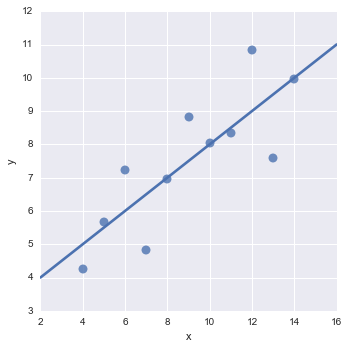
\includegraphics[width=0.7\linewidth]{images/regression_19_0}
\end{figure}

\end{frame}

%=========================================%
\begin{frame}[fragile]
\large	
The linear relationship in the second dataset is the same, but the plot clearly shows that this is not a good model:
\begin{framed}
	\begin{verbatim}
sns.lmplot(x="x", y="y", data=anscombe.query("dataset == 'II'"),
           ci=None, scatter_kws={"s": 80});
                  \end{verbatim}
                \end{framed}
\begin{figure}
	\centering
	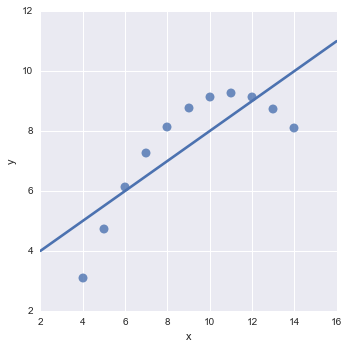
\includegraphics[width=0.7\linewidth]{images/regression_21_0}

\end{figure}


\end{frame}


%=========================================%
\begin{frame}[fragile]
	\large	
In the presence of these kind of higher-order relationships, \texttt{lmplot()} and \texttt{regplot()} can fit a polynomial regression model to explore simple kinds of nonlinear trends in the dataset:
\begin{framed}
	\begin{verbatim}
sns.lmplot(x="x", y="y", data=anscombe.query("dataset == 'II'"),
           order=2, ci=None, scatter_kws={"s": 80});
               \end{verbatim}
            \end{framed}
\begin{figure}
	\centering
	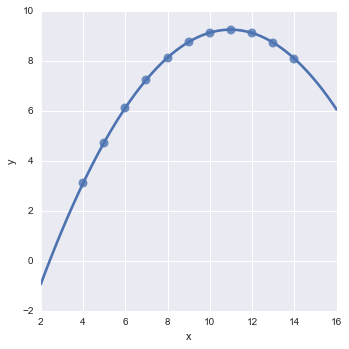
\includegraphics[width=0.7\linewidth]{images/regression_23_0}

\end{figure}

\end{frame}
%=========================================%
\begin{frame}[fragile]
	\large
A different problem is posed by “outlier” observations that deviate for some reason other than the main relationship under study:
\begin{framed}
\begin{verbatim}
sns.lmplot(x="x", y="y", data=anscombe.query("dataset == 'III'"),
           ci=None, scatter_kws={"s": 80});
               \end{verbatim}
            \end{framed}
\begin{figure}
	\centering
	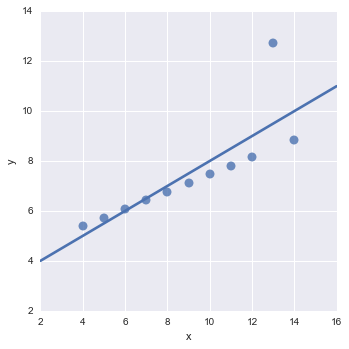
\includegraphics[width=0.7\linewidth]{images/regression_25_0}
\end{figure}


\end{frame}
%=========================================%
\begin{frame}
In the presence of outliers, it can be useful to fit a robust regression, which uses a different loss function to downweight relatively large residuals:
\begin{framed}
\begin{verbatim}
sns.lmplot(x="x", y="y", data=anscombe.query("dataset == 'III'"),
           robust=True, ci=None, scatter_kws={"s": 80});
               \end{verbatim}
            \end{framed}
\begin{figure}
	\centering
	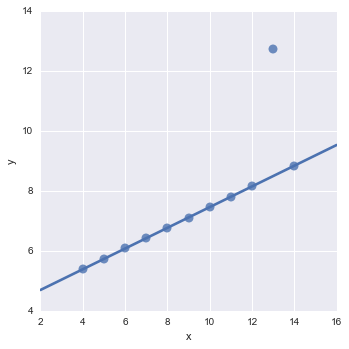
\includegraphics[width=0.7\linewidth]{images/regression_27_0}

\end{figure}
\end{frame}
%=========================================%
\begin{frame}[fragile]
When the y variable is binary, simple linear regression also “works” but provides implausible predictions:
\begin{verbatim}
tips["big_tip"] = (tips.tip / tips.total_bill) > .15
sns.lmplot(x="total_bill", y="big_tip", data=tips,
           y_jitter=.03);
        \end{verbatim}
\begin{figure}
	\centering
	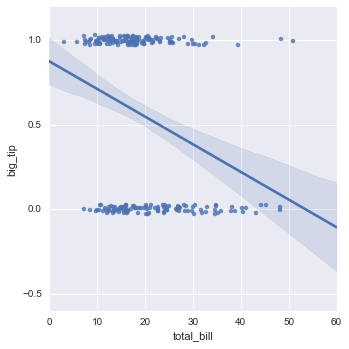
\includegraphics[width=0.7\linewidth]{images/regression_29_0}
\end{figure}

\end{frame}
%=========================================%
\begin{frame}[fragile]
The solution in this case is to fit a logistic regression, such that the regression line shows the estimated probability of y = 1 for a given value of x:
\begin{verbatim}
sns.lmplot(x="total_bill", y="big_tip", data=tips,
           logistic=True, y_jitter=.03);
          \end{verbatim}
\begin{figure}
	\centering
	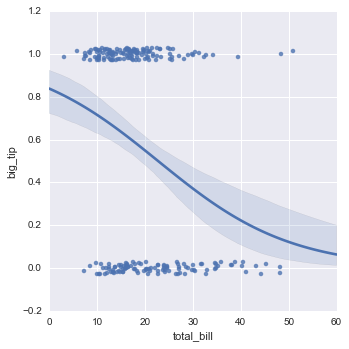
\includegraphics[width=0.7\linewidth]{images/regression_31_0}
\end{figure}
\end{frame}
%===========================================================%
\begin{frame}
\large
\begin{itemize}
\item Note that the logistic regression estimate is considerably more computationally intensive (this is true of robust regression as well) than simple regression, and as the confidence interval around the regression line is computed using a bootstrap procedure, you may wish to turn this off for faster iteration (using \texttt{ci=False}).
\item An altogether different approach is to fit a nonparametric regression using a lowess smoother. This approach has the fewest assumptions, although it is computationally intensive and so currently confidence intervals are not computed at all:
\end{itemize}


\end{frame}
%==============================================%
\begin{frame}[fragile]
	\large
	\begin{framed}
\begin{verbatim}
sns.lmplot(x="total_bill", y="tip", data=tips,
           lowess=True);
           \end{verbatim}
        \end{framed}
\begin{figure}
	\centering
	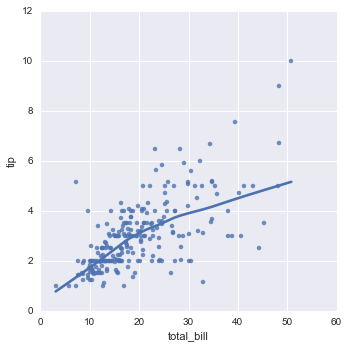
\includegraphics[width=0.7\linewidth]{images/regression_33_0}
\end{figure}

\end{frame}
%==============================================%
\begin{frame}[fragile]
	\large
	

The \texttt{residplot()} function can be a useful tool for checking whether the simple regression model is appropriate for a dataset. It fits and removes a simple linear regression and then plots the residual values for each observation. Ideally, these values should be randomly scattered around y = 0:

\begin{verbatim}
sns.residplot(x="x", y="y", data=anscombe.query("dataset == 'I'"),
scatter_kws={"s": 80});
\end{verbatim}

\begin{figure}
	\centering
	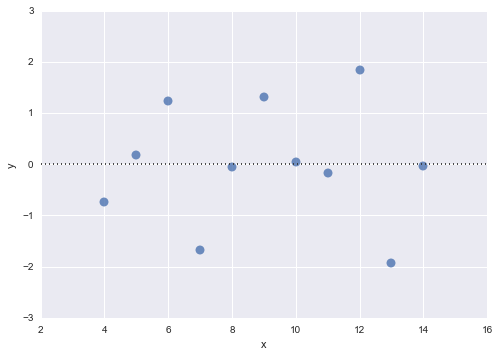
\includegraphics[width=0.7\linewidth]{images/regression_35_0}
\end{figure}
\end{frame}
%==============================================%
\begin{frame}[fragile]
	\large
If there is structure in the residuals, it suggests that simple linear regression is not appropriate:
\begin{verbatim}
sns.residplot(x="x", y="y", data=anscombe.query("dataset == 'II'"),
              scatter_kws={"s": 80});
\end{verbatim}
\begin{figure}
\centering
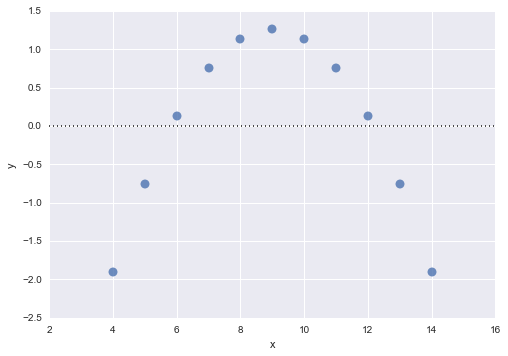
\includegraphics[width=0.7\linewidth]{images/regression_37_0}
\end{figure}

\end{frame}
\end{document}